\section{Overview of Causal Graphs}

Causal diagrams and causal graphical models have been introduced by Pearl 
(2000) as a powerful tool for causal inference, especially in observational 
studies. Perhaps one of the most important and useful features of causal 
graphs when dealing with causal inference problems is the clear illustration 
of the causal relationships between the variables. 
While a formal introduction to the topic of directed acyclic graphs (DAGs) is beyond the scope of this chapter, 
here we focus specifically on illustrating the power of DAGs to represent 
and encode complex  causal relationships between variables in an intuitive and 
clear manner. Interested readers can refer to Pearl (2000) for a thorough introduction. 


Consider the causal graph represented in Figure \ref{fig:simple-graph}. Suppose we're interested 
in the effect of Z on Y. What the graph in Figure \ref{fig:simple-graph} implies is that Z is 
independent of Y(Z) given X, or in other words, the assignment mechanism is 
ignorable conditional on the values of X [TODO: insert equations for the 
ignorability assumption]. In such situations, it is sufficient to control for 
X to obtain an unbiased estimate of the causal effect of Z on Y. 

\begin{figure}
   \centering
   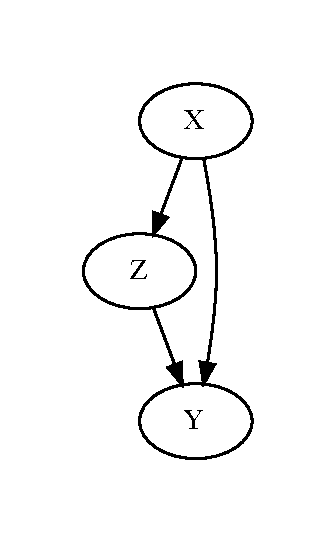
\includegraphics[width=0.5\textwidth]{simple-graph.pdf}
   \caption{Simple DAG of the causal relationships between X, Y and Z}
   \label{fig:simple-graph}
\end{figure}

Now note the set of structural equations needed to convey the same assumptions as figure bla. 
\[Z = f_Z(X, \epsilon_Z)  \]

\[Y(z) = f_Y(X, z, \epsilon_Y)  \]

Now consider the case where there exists another latent confounding variable, U, which also affects both the treatment Z, as well as the outcome, Y. Figure \ref{fig:simple-graph-confounded} illustrates this assumption in DAG form, and the equations below are the structural equation equivalent:

\[Z = f_Z(X, U, \epsilon_Z)  \]

\[Y(z) = f_Y(X, U, z, \epsilon_Y)  \]

\begin{figure}
   \centering
   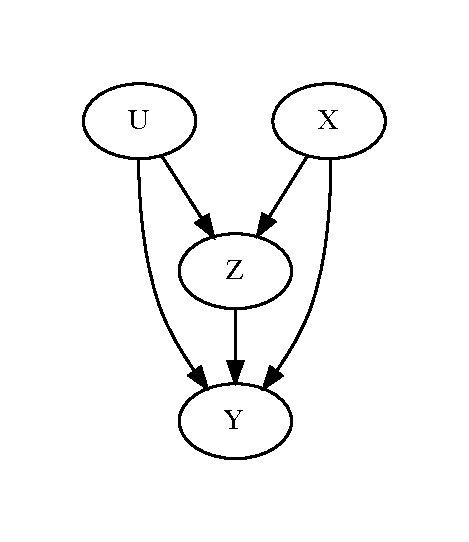
\includegraphics[width=0.5\textwidth]{simple-graph-confounded.pdf}
   \caption{Simple DAG of the causal relationships between X, Y and Z and confounder U}
   \label{fig:simple-graph-confounded}
\end{figure}

It is clear from Figure \ref{fig:simple-graph-confounded} that conditioning on X alone does not block all the indirect paths between Z and Y, and thus ommitting it 
will yield biased results of the causal relationship between Z and Y. The structural equations also show that the ignorability assumption 
of Z does not hold if we only condition on X, and we risk obtaining biased estimates of the causal effect of Z on Y if we fail to 
account for U. 

Even in this very simple example with only three or four variables, one can see the advantage of using a causal graph to encode assumptions. 
This advantage of DAGs becomes even more apparent in larger problems with many covariates available, and where the causal structure of the data is way more complicated, which are the types of problems typically faced by transportation demand modelers. 



Lastly, it is important to note that the graphical approach to causality focuses 
primarily on issues of identification of causal effects, that is, given a 
directed acyclic graph (DAG) that encodes an analyst's knowledge and belief 
about the data generation process of the problem at hand, can a specific 
causal effect be identified? As such, we emphasize that DAGs are great tools 
for a modeler to encode their assumptions about a problem, but not necessarily 
a guide on how to estimate a causal effects of interest. However, DAGs come 
with a set of testable implications, and incorporating them in any causal 
analysis adds robustness and defensibility to one's analysis. 





